%
% path-finding
% @author Tobias Weber <tweber@ill.fr>
% @date 2021
% @license see 'LICENSE' file
%

\chapter{Path-finding Details and Implementation}
\label{ch:impl}

In this chapter we describe the individual steps of the strategy (see p. \pageref{sec:strategy}) in detail
and present an implementation in C++ \cite{Stroustrup2008, Stroustrup2018}. Specifically,
the latest version 20 of the C++ standard \cite{ISOCPP20} was employed in the creation of the software
together with the Boost C++ template libraries \cite{web_boost}. The source code for the implementation
can be found in the directory \lstinline|./src/core| together with the library routines in \lstinline|./src/libs|
of the repository at \url{https://code.ill.fr/scientific-software/takin/paths}. Stable versions of the
source code have furthermore been registered under the DOI \href{https://doi.org/10.5281/zenodo.4625649}{10.5281/zenodo.4625649}.

Section \ref{sec:tasmodel} is dedicated to modelling the triple-axis spectrometer (TAS), 
section \ref{sec:buildpath} discusses the steps involved in building up the instrument path, 
and section \ref{sec:exepath} focuses on executing the instrument motion along the path.
The graphical user interface is presented separately, namely in chapter \ref{ch:gui}.





% -----------------------------------------------------------------------------
% instrument model
% -----------------------------------------------------------------------------
\section{TAS instrument modelling}
\label{sec:tasmodel}

The instrument space comprising the triple-axis spectrometer, the walls and obstacles as well as the floor is modelled in
the class \lstinline[language=C++]|InstrumentSpace|. It also serves as high-level interface for loading and saving
the instrument geometry and states, signalling mechanisms for state changes using the publish-subscribe mechanism
via \textit{Boost.Signals2} \cite{web_boost_signals}, as well as checking the instrument for collisions.

The classes \lstinline[language=C++]|Instrument| and \lstinline[language=C++]|Axis| contain the actual instrument definition.
The spectrometer is modelled as a hierarchy of the three principal axes, namely monochromator, sample and analyser.
Each axis has three local coordinate systems, namely the rotation relative to the incoming and outgoing vector, respectively,
and an internal rotation which is decoupled from the other local rotations.
Geometrical objects are derived from the abstract, purely virtual class \lstinline[language=C++]|Geometry| and can be
coupled to any of these three local coordinate systems.
This makes it possible to model neutron-optical components attached to the either the incoming or outgoing path of the
neutron beam at the specific axis. It furthermore makes it possible to have components which rotate independently of
the axis.
Physically, the outgoing coordinate system is equal to the scattering angle, while the internal angle corresponds
to the crystal rocking angle (see Ch. \ref{ch:xtal}).
The transformation matrices corresponding to the three local coordinate systems are calculated as follows:

\begin{equation}
\begin{split}
	T_{\mathrm{in}}^{i} & \ =\  T_{\mathrm{out}}^{i-1} \cdot P^{i} \cdot R\left(\theta_{\mathrm{in}}^{i}\right), \\
	T_{\mathrm{int}}^{i} & \ =\  T_{\mathrm{in}}^{i} \cdot R\left(\theta_{\mathrm{int}}^{i}\right), \\
	T_{\mathrm{out}}^{i} & \ =\  T_{\mathrm{in}}^{i} \cdot R\left(\theta_{\mathrm{out}}^{i}\right).
\end{split}
\end{equation}

Here, $T_{\mathrm{in,\, int,\, out}}^{i}$ names the transformation matrices of the incoming, internal (decoupled) and outgoing
coordinate system of axis $i$, respectively.
$T_{out}^{i-1}$ is the outgoing transformation of the preceding instrument axis, or the identity if it is the first axis in the hierarchy.
$R\left(\theta_{\mathrm{in,\, int,\, out}}\right)$ are the corresponding rotation matrices and $P^i$ is the translation
of the local coordinate origin of the respective axis $i$.
The situation is depicted in Fig. \ref{fig:tas_axes}.


\begin{figure*}
	\begin{minipage}{0.45 \textwidth}
		\begin{center}
			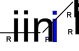
\includegraphics[width = 0.75 \textwidth]{figures/axis}
		\end{center}
	\end{minipage}
	%\hspace{1cm}
	\begin{minipage}{0.45 \textwidth}
		\begin{center}
			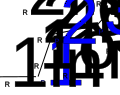
\includegraphics[width = 0.95 \textwidth]{figures/axes}
		\end{center}
	\end{minipage}
	\caption{Left panel: Local transformations for an axis. The symbols $R_{\mathrm{x}}^i$ are shorthands
	for the rotation matrices $R\left( \theta_{\mathrm{x}}^i \right)$, with $x = \left\{ \mathrm{in,\, int,\, out} \right\}$.
	$P^i$ is the point of origin for the axis.
	Right panel: Three coupled axes build up the triple-axis spectrometer, with axes 1, 2, and 3 naming the monochromator,
	the sample, and the analyser axis, respectively.
	\label{fig:tas_axes}}
\end{figure*}

% -----------------------------------------------------------------------------





% -----------------------------------------------------------------------------
% path building
% -----------------------------------------------------------------------------
\section{Path-building}
\label{sec:buildpath}

As discussed in chapter \ref{sec:tasrobot}, path-creation will be based on the angular configuration space
(as opposed to -- for example -- crystal configuration space). The top-level C++ class for creating the path
is named \lstinline[language=C++]|PathBuilder|. It mainly calls the low-level routines from the geometry
library situated in the directory \lstinline|./src/libs| of the source code repository.


\subsection{Angular configuration space}
As the obstacles do not have any geometrically primitive shape in angular configuration space, we iterate
through the configuration space on a two-dimensional grid and create a bitmap of allowed and forbidden
positions. The grid extends towards the scattering angles $2\theta_S \in \left[ -180^{\circ},\, 180^{\circ} \right]$
and monochromator angles of $2\theta_M \in \left[0^{\circ},\, 180^{\circ} \right]$, where, for the monochromator, we do
not the full angular range as this is not possible in real instruments which has the monochromator at a fixed position
and only scatters in one direction. The sample scattering angle, on the other hand, needs the full angular range as
scattering on both sides of the axis is done in practice.

To check for the allowed positions, the instrument model as described in sec \ref{sec:tasmodel} is moved to
each $\left( 2\theta_S,\, 2\theta_M \right)$ position on the grid and tested for collisions with the walls or with
itself. Even though the instrument model itself is a three-dimensional representation of the spectrometer, we
can nevertheless simplify the collision detection checks to a two-dimensional plane. The reason for this is
that all possible obstacles in the instrument path, for instance walls and pillars, are upright and do not have
any sloped angles. The same is true for the instrument itself.
The collision calculation on the two-dimensional grid is spread out on several processor cores using 
the \lstinline[language=C++]|thread_pool| \cite{web_boost_asio_threadpool} class from the 
\textit{Boost.Asio} \cite{web_boost_asio} asynchronous input/output library.

With the given two-dimensional simplifications, we only need to distinguish three possible intersection tests for collisions: 
line-line intersections, line-circle intersections and circle-circle intersections. 
For efficiency, the actual calculations are only made if the corresponding geometrical objects lie within 
one another's axis-aligned bounding boxes \cite{web_aabb}.

\subsubsection*{Line-line intersections}
Given two lines $\left|x_1\right> + \lambda_1 \left|d_1\right>$ and $\left|x_2\right> + \lambda_2 \left|d_2\right>$, 
the line-line intersection can be calculated by setting their equations equal, namely as follows \cite{wiki_line_line_intersection}:
\begin{equation}
	\left|x_1\right> + \lambda_1 \left|d_1\right> \ =\ \left|x_2\right> + \lambda_2 \left|d_2\right>,
\end{equation}
\begin{equation}
	\left|x_1\right> - \left|x_2\right> \ =\  \lambda_2 \left|d_2\right> - \lambda_1 \left|d_1\right>,
\end{equation}
\begin{equation}
	\left|x_1\right> - \left|x_2\right> \ =\  D \cdot \left| \lambda \right>,
	\label{eq:line_line_inters}
\end{equation}
where, in the last step, the matrix $D$ is composed of the direction vectors in its columns, $D = \left( d_2 \ |\  -d_1 \right)$, 
and the vector $\left| \lambda \right>$ has the two individual line parameter $\lambda_1$ and $\lambda_2$ in its
rows, $\left| \lambda \right> = \left( \lambda_2 \ |\  \lambda_1 \right)^T$.

For the given two-dimensional case, one can now directly solve for the $\lambda$s by left-multiplying with $D^{-1}$.
As the routine is also used by other code parts, we also include the general $n$-dimensional case in the implementation, 
determining the closest point between the two lines if no intersection exists.
This is done using the normal equation of the least-squares problem \cite[p. 793]{Arens2015}; 
the approximate version of Eq. \ref{eq:line_line_inters} thus reads \cite{wiki_line_line_intersection}: 
\begin{equation}
	D^T \left(\left|x_1\right> - \left|x_2\right>\right) \ =\  D^T D \cdot \left| \lambda \right>,
\end{equation}
\begin{equation}
	\left| \lambda \right> \ =\  \left( D^T D \right)^{-1} D^T \cdot \left( \left|x_1\right> - \left|x_2\right> \right).
\end{equation}

The intersection point (or the closest point) is thus be found by inserting the $\lambda$ parameters in the respective line equation. 
Testing for the intersection of line segments instead of infinite lines is done by keeping the $\lambda$ parameters inside a given range.

For an efficient handling of multiple line segment intersections, the decision for which lines to test for intersections is
performed using the line segment sweep algorithm from Ref. \cite[pp. 69-80]{FUH_geo2020} whose C++ implementation can be
found in the function \lstinline[language=C++]|intersect_sweep| of the file \lstinline|./src/libs/lines.h|.
We shortly summarise the algorithm and our implementation, following the description in \cite[pp. 69-80]{FUH_geo2020}:
\begin{enumerate}
	\item Possible events are kept in an event structure. Before the sweep, this is initialised with all the line segment
		endpoints. The structure itself is a priority queue which sorts its elements by their $x$ coordinate in ascending order.
		In the implementation we use the \lstinline[language=C++]|std::priority_queue| of the C++ standard library.
	\item The line sweep is performed by iteratively taking the top element from the event structure's priority queue until
		the latter is empty, in which case the algorithm terminates.
		Depending on the type of the current element on top of the event structure, the following actions are performed:
		\begin{itemize}
			\item If the current event is the left endpoint of a line segment, the newly encountered line segment is
				inserted into the sweep status structure and is tested for intersections against its preceding and succeeding
				line segment in the status structure. Potential intersections are inserted into the event structure.
				The sweep status structure sorts the line segments according to their $y$ order at the current $x$ position
				of the sweep line. It is implemented using \textit{Boost.Intrusive}'s \cite{web_boost_intrusive}
				AVL tree class \cite{web_boost_intrusive_avltree} and can be found in the file \lstinline|./src/libs/trees.h|.
			\item If the current event is the right endpoint of a line segment, the now inactive line segment is
				removed from the sweep status structure and its preceding and succeeding line segments are tested
				for intersection. A potential intersection is inserted into the event structure.
			\item If the current event is an intersection point, the involved line segments are reported as intersecting
				and, as they cross at this point, their order is flipped in the event structure.
				After the flip, the intersecting line segments are tested against intersection with their new neighbours
				and the possible intersection points are inserted into the event structure.
		\end{itemize}
	\item Repeat from step 2.
\end{enumerate}


\subsubsection*{Line-circle intersections}
As with the line-line intersection, we keep the problem general and directly look at the $n$-dimensional problem.
The intersection points between a line and an $n$-sphere are found by inserting the line equation 
$\left|p\right> = \left|x_1\right> + \lambda \left|d\right>$ into the sphere equation 
$\left< p-x_2 \ |\  p-x_2 \right> = r^2$, where $x_1$ names an arbitrary point on the line, $d$ its normalised 
direction vector, $x_2$ is the centre of the sphere/circle, and $r$ its radius \cite{wiki_line_sphere_intersection}.
The intersection points along the line are thus given by \cite{wiki_line_sphere_intersection}:
\begin{equation}
	\lambda \ =\ \left< x_2 - x_1 \  |\  d \right>
		\ \pm\ \sqrt{ \left< x_2 - x_1 \  |\  d \right>^2 
			+ r^2 - \left< x_2 - x_1 \ |\  x_2 - x_1 \right>}.
\end{equation}



\subsubsection*{Circle-circle intersections}
In this case we do not need the actual intersection points, so the calculation is restricted to calculation if
the circles overlap. This is the case when the distance of their centres $\left| x_1 \right>$ and $\left| x_2 \right>$ 
is less than the sum of their radii, $r_1$ and $r_2$, respectively:

\begin{equation}
	\left< x_2 - x_1 \ |\ x_2 - x_1  \right> \ \leq \ \left( r_2 + r_1 \right)^2.
\end{equation}



\subsection{Contour tracing}
\label{sec:contourtracing}
Having determined a bitmap representation of allowed and forbidden regions in the angular configuration space,
we now need to trace the boundary contour between these regions.
To this end we use the radial sweep algorithm \cite{web_radial_sweep} whose implementation can be found
in the function \lstinline[language=C++]|trace_boundary| located in the file \lstinline|./src/libs/img.h|.

The radial sweep algorithm works as given below, following the descriptions in Ref. \cite{web_radial_sweep}:
\begin{enumerate}
	\item Scan the bitmap line by line and row by row until a forbidden region is found. 
		If the corresponding pixel has already been seen, continue. Otherwise mark it as start pixel.
	\item Set an arbitrary direction vector pointing to one of the eight neighbouring pixels.
	\item Rotate the direction vector in a given, fixed sense, i.e. either in an always clockwise or 
		always counter-clockwise fashion, until the pixel it points to is again inside a forbidden region.
		If a full rotation has been performed without hitting a new forbidden region, stop the algorithm.
	\item Increment the current pixel position using the newly found direction vector. 
		Set the new direction vector to point from the new pixel to the old one.
		Add the line connecting the old and the new pixel to the boundary.
	\item Repeat from step 3 until the start pixel is seen again (or no new direction vector is found).
\end{enumerate}



\subsection{Line-segment generation and simplification}

After creating the line segments from the traced contour lines, they have to be cleaned up and simplified,
because the quantity of superfluous vertices would considerably slow down the generation of the Voronoi 
diagram in one of the next steps.
In the function \lstinline[language=C++]|simplify_contour|, which resides in the file \lstinline|./src/libs/hull.h|,
we perform two simplification steps:

First, ``staircase artefacts'' are removed. These kinds of artefacts originate from tracing diagonal or sloped lines.
The quantification of the obstacles on a grid and the subsequent run of the contour tracer (section \ref{sec:contourtracing})
create a succession of horizontal and vertical line segments in lieu of the actual diagonal.
The first simplification step looks for these line segments and replaces them with proper diagonal lines.

A second simplification step replaces collections of short collinear line segments with larger ones.
To that end, we iterate through the vertices on the contour line and remove any vertices whose line segment angles 
involving the previous and the next vertex, respectively, are below a given epsilon value.



\subsection{Generation of convex regions}
\label{sec:convex_regions}




\subsection{Calculation of the Voronoi diagram}
As we are interested in the instrument path that is at the farthest position from walls, we need to calculate
the Voronoi diagrams for the line segments that constitute these obstacles. In a second step, we group line
segments into objects in to remove bisecting lines coming from the same object.


\subsubsection*{Line segment Voronoi diagrams}
Voronoi diagrams are described in a general fashion in \cite[Ch. 7, pp. 147f]{Berg2008} and in
\cite[Ch. 5, pp. 209f]{Berg2008}, a description of the special case of Voronoi diagrams for line segments can be
found in \cite[Ch. 7.3, pp. 160-163]{Berg2008} and in \cite[pp. 242-247]{FUH_geo2020}.

The Voronoi region of a line $l_i$ consists of all points in $\mathbb{R}^2$ that are closest to $l_i$. 
The boundary between the Voronoi regions of two line segments $l_i$ and $l_j$, $i \neq j$ , 
is called bisector and is the curve of equal distance between the two line segments $l_i$ and $l_j$.
Its shape is either linear or quadratic, where, in the linear case, the bisector curve can also be either
finite or infinite \cite[pp. 243-244]{FUH_geo2020}.

A linear bisector is obtained for the distance calculated between two line segment endpoints or between two inner 
points on the line segments which are not the endpoints.
This can easily be seen, because, (a) in the case of two endpoints, the middle perpendicular line between these 
two points is equidistant to them; and (b) in the case of two line segments, the angular bisector of the two lines is
equidistant to them \cite[pp. 243-244]{FUH_geo2020}.
On the other hand, the bisector curve segment follows a parabolic shape if the distance is calculated 
between a line segment endpoint and one inner point of the other segment. This is the same as the bisector between
a point and a line and it parabolic distance is shown in \cite[pp. 260-261]{FUH_geo2020}.
An example of two or several line segments and their bisectors is shown in Fig. \ref{fig:linesegs_voro}.

For the calculation of the line segment Voronoi diagrams in the present implementation, the Voronoi extensions
\cite{web_boost_polygon_voronoi} of the \textit{Boost.Polygon} \cite{web_boost_polygon, Simonson2009} C++ library are used.
\textit{Boost.Polygon} uses Fortune's sweep algorithm \cite{Fortune1987} to construct the Voronoi diagram and is
internally based on integers coordinates \cite{web_boost_polygon}.
The reliance on integer coordinate representation is also responsible for \textit{Boost.Polygon}'s inability to handle
intersecting lines, because the intersection point may be at a non-integer coordinate. Intersecting lines need
to be carefully filtered out, because they can cause the library to either crash, hang, or yield wrong bisectors.

Several alternative libraries for calculating the line segment Voronoi diagrams exist,
noteworthy are \textit{VRONI} by M. Held \cite{Held2001}, \textit{OpenVoronoi} by A. E. Wallin \cite{web_openvoronoi}
and \textit{VoroLS} by W. Schumann \cite{DiplomaSchumann}.
A further possible C/C++ library, the popular and very high-quality \textit{QHull} by C. B. Barber \cite{web_qhull},
only calculates the Voronoi diagrams for vertices, not for line segments.
None of the above is feasible for the present project, though: \textit{VRONI} is neither freely available nor under a
suitable open-source license.
The opposite is true for \textit{OpenVoronoi}: It is available under an open-source license, but our first tests
deemed it too unstable for use in a production-quality software. The source code for our test can be found in
the function \lstinline[language=C++]|calc_voro_ovd|, which resides in file \lstinline|./src/libs/hull.h|.
The source code for the test tool itself is located in: \lstinline|./src/tools/lines.cpp|.
\textit{VoroLS} is stable and does even handle intersecting lines, but is a \textit{Java}
software, not a library, and is not under an open-source license.


\label{sec:voronoi}
\begin{figure*}
	\begin{minipage}{1 \textwidth}
		\begin{center}
			\includegraphics[width = 0.75 \textwidth]{figures/linesegs}
		\end{center}
		\vspace{0.25cm}
	\end{minipage}
	\begin{minipage}{1 \textwidth}
		\vspace{0.25cm}
		\begin{center}
			\includegraphics[width = 0.95 \textwidth]{figures/linesegs2}
		\end{center}
	\end{minipage}
	\caption{Top panel: Voronoi regions for two line segments, $l_1$ and $l_2$.
		Bottom panel: Voronoi regions for five line segments, $l_1,\, l_2,\, ...,\, l_5$.
		The line segments and their endpoints are marked in blue. The small red points represent the Voronoi vertices.
		The black lines are the bisectors of the Voronoi regions, where the solid lines delimit finite and the dashed lines
		infinite regions. Helper lines are marked in red. The figure has been calculated using the \textit{Boost.Polygon} library
		\cite{web_boost_polygon_voronoi} and the source code in \lstinline|./src/tools/lines.cpp|.
		\label{fig:linesegs_voro}}
\end{figure*}



\subsubsection*{Polygon Voronoi diagrams}

It is not sufficient to represent the walls as isolated line segments, because -- 
as we saw before -- they are not necessarily simply-connected. 
We rather represent them as concave or convex regions, of which we group all 
line segments that form the boundary of a simply-connected region.

The Voronoi diagrams only need to be calculated between such regions, 
the bisectors from line segments belonging to the same region are discarded. 
Fig. \ref{fig:linesegs_grouped_voro} shows an example of line segments and several
possibilities of grouping them. 
In case (a) they are not grouped and the Voronoi diagram is just the line 
segment Voronoi diagram. This case cannot be used for the paths of the spectrometer,
since the bisectors enter the forbidden region inside a wall.
In case (b) collections of line segments, which form arbitrary concave polygons, 
are grouped grouped into regions. Here, the bisectors do not touch any region 
and the resulting path is what is called the ``contour-parallel tool path'' in 
the terms of CNC (computer numerical control) milling machines \cite{Jeong1998, wiki_milling}, where these are utilised. While the bisectors of this case could 
be used for the spectrometer path mesh, a problem remains: In contrast to a milling
machine the spectrometer is not supposed to be at the furthest distance of any
polygonal region at all times, but has a starting and ending position which can 
be close to one of these walls or be at a position near a concave corner which
is not directly accessible from the present bisector configuration. This problem
is solved in case (c).
In case (c) the concave polygonal regions are split into convex sub-regions, see
section \ref{sec:convex_regions}.
The bisectors form what is called a skeletal bisector configuration [TODO: cite].
Here, each part of the instrumental configuration space can be reached from the
bisector mesh and no bisectors inside forbidden regions exits. This configuration
will be used in the software for calculating the bisector path mesh for instrument
movement.

In the implementation we distinguish between contours and inverted contours, with 
the former enclosing forbidden regions (and having an open allowed region outside) 
and the latter enclosing allowed regions (and having an open disallowed region outside).
This is a purely technical detail as mathematically the two cases are the same
with just the turning sense of the contour being different. 
Due to the nature of the contour-tracing algorithm (see section \ref{sec:contourtracing}), 
the turning sense of the contour is not preserved, and the nature of the contour 
and its regions have to be determined and stored separately.
Panel (c) of Fig. \ref{fig:linesegs_grouped_voro} shows the distinction: 
The contour of region 1 is an inverted one, as it encloses an allowed region,
whereas regions 2 and 3 are non-inverted, meaning they enclose forbidden regions.

The collection of normal and inverted regions is calculated in the member function
\lstinline[language=C++]|CalculateLineSegments| of the \lstinline[language=C++]|PathsBuilder|
class, which resides in file \lstinline|./src/core/PathsBuilder.cpp|. 
The Voronoi diagram of these regions is calculated in the member function
\lstinline[language=C++]|PathsBuilder::CalculateVoronoi|.


\label{sec:voronoi}
\begin{figure*}
	\begin{minipage}{0.5 \textwidth}
		\begin{center}
			\includegraphics[width = 1 \textwidth]{figures/linesegs_ungrouped}
		\end{center}
	\end{minipage}
	\begin{minipage}{0.5 \textwidth}
		\begin{center}
			\includegraphics[width = 1 \textwidth]{figures/linesegs_grouped}
		\end{center}
	\end{minipage}
	\begin{minipage}{0.5 \textwidth}
		\begin{center}
			\includegraphics[width = 1 \textwidth]{figures/linesegs_skeleton}
		\end{center}
	\end{minipage}
	\caption{Panel (a): Ungrouped line segments and their Voronoi bisectors.
		Panel (b): The same line segments, but with each polygonal region grouped.
		The Voronoi diagram is only calculated between groups, not within the same group.
		Panel (c): A mixture of the first two cases, where not entire regions are grouped
		as in case (b), but where each convex sub-region forms its own group.
		\label{fig:linesegs_grouped_voro}}
\end{figure*}



% -----------------------------------------------------------------------------





% -----------------------------------------------------------------------------
% instrument motion
% -----------------------------------------------------------------------------
\section{Instrument movement}
\label{sec:exepath}


\subsection{Determination of the start and end coordinates}



\subsection{Calculation of Dijkstra's shortest path}
\label{sec:dijkstra}


% -----------------------------------------------------------------------------
